Schéma objet-relationnel / 100\% relationnel.

Discussion sur pourquoi 100\% relationnel ?! ORM ?! Doctrine / Symfony ?

Présentation des templates / formulaires

\section{Paradigme}
Le choix du paradigme est crucial. Objet? Objet-relationnel ou relationnel pur?

\subsection{Le paradigme objet}

Le modèle objet pour le stockage des données présente les mêmes avantages que pour la programmation orienté objet, à savoir
une grande capacité d'abstraction, de factorisation et de maintenance. Malheureusement ce paradigme n'est que peu implémenté 
par les SGBD (O2, db4o, ObjectStore) ce qui nuit grandement à la portabilité d'une application basé sur ce paradigm.

\subsection{Le paradigme objet-relationnel}

De nombreux SGBD tels que ORACLE offrent un paradigme hybride entre l'objet et le relationnel, l'objet-relationnel.
Ce paradigme est standardisé par la norme SQL3 cependant celle-ci n'est jamais implémentée dans sa globalité
ce qui pose à nouveau un problème de portabilité (un script SQL pour ORACLE ne s'exécutera pas sur PostgreSQL et vice-versa).

\subsubsection{Schéma objet-relationnel}
\lstinputlisting[language=sql]{./sources/schema_objet_relationnel.sql}

\subsection{Le paradigme relationnel pur}

Le paradigme relationnel pur est le paradigme historique des bases de données, il offre des performances reconnus. Par contre,
l'utilisation de ce paradigme demande de manipuler deux schémas de données différents, celui de la base de données et celui de
la partie programmation qui est objet.

\subsubsection{Schéma relationnel}
\begin{description}
\item[TERME](\underline{lib\_terme})
\item[CONCEPT](\underline{terme\_vedette}\up{\#}, concept\_general\up{\#})
\item[SYNONYME](\underline{terme\up{\#}, concept\up{\#}})
\item[ASSOCIATION](\underline{concept1\up{\#}, concept2\up{\#}})
\end{description}

\section{ORM}

	\subsection{Qu'est qu'un ORM?}
    Un ORM ou mapping objet-relationnel (en anglais object-relational mapping ou ORM) est outil informatique qui crée l'illusion d'une base de données orientée objet à partir d'une base de données relationnelle en servant d'interface entre celle-ci et le code de l'application. On pourrait le traduire par \og correspondance entre paradigme objet et paradigme relationnel \fg.
   
	\subsection{Pourquoi?}
    Nous avons vu que les systèmes de gestion de base de données orientées objet sont actuellement peu nombreuses,
    que la norme SQL3 n'est que très partiellement implémenté. Nous avons donc choisi de rester sur un valeur sûr,
    le relationnel pur. Par contre, ce paradigme présente le désavantage d'un schéma différents et donc d'un effort
    de programmation supplémentaire et redondant pour adapter chaque objet de notre code vers sa représentation
    dans la base de données. Or, les ORM propose de faire se travail à notre place.

	\subsection{Décisions}
	
	
\subsection{Templates et formulaires}

\subsubsection{Accueil}
\begin{figure}[H]
\begin{center}
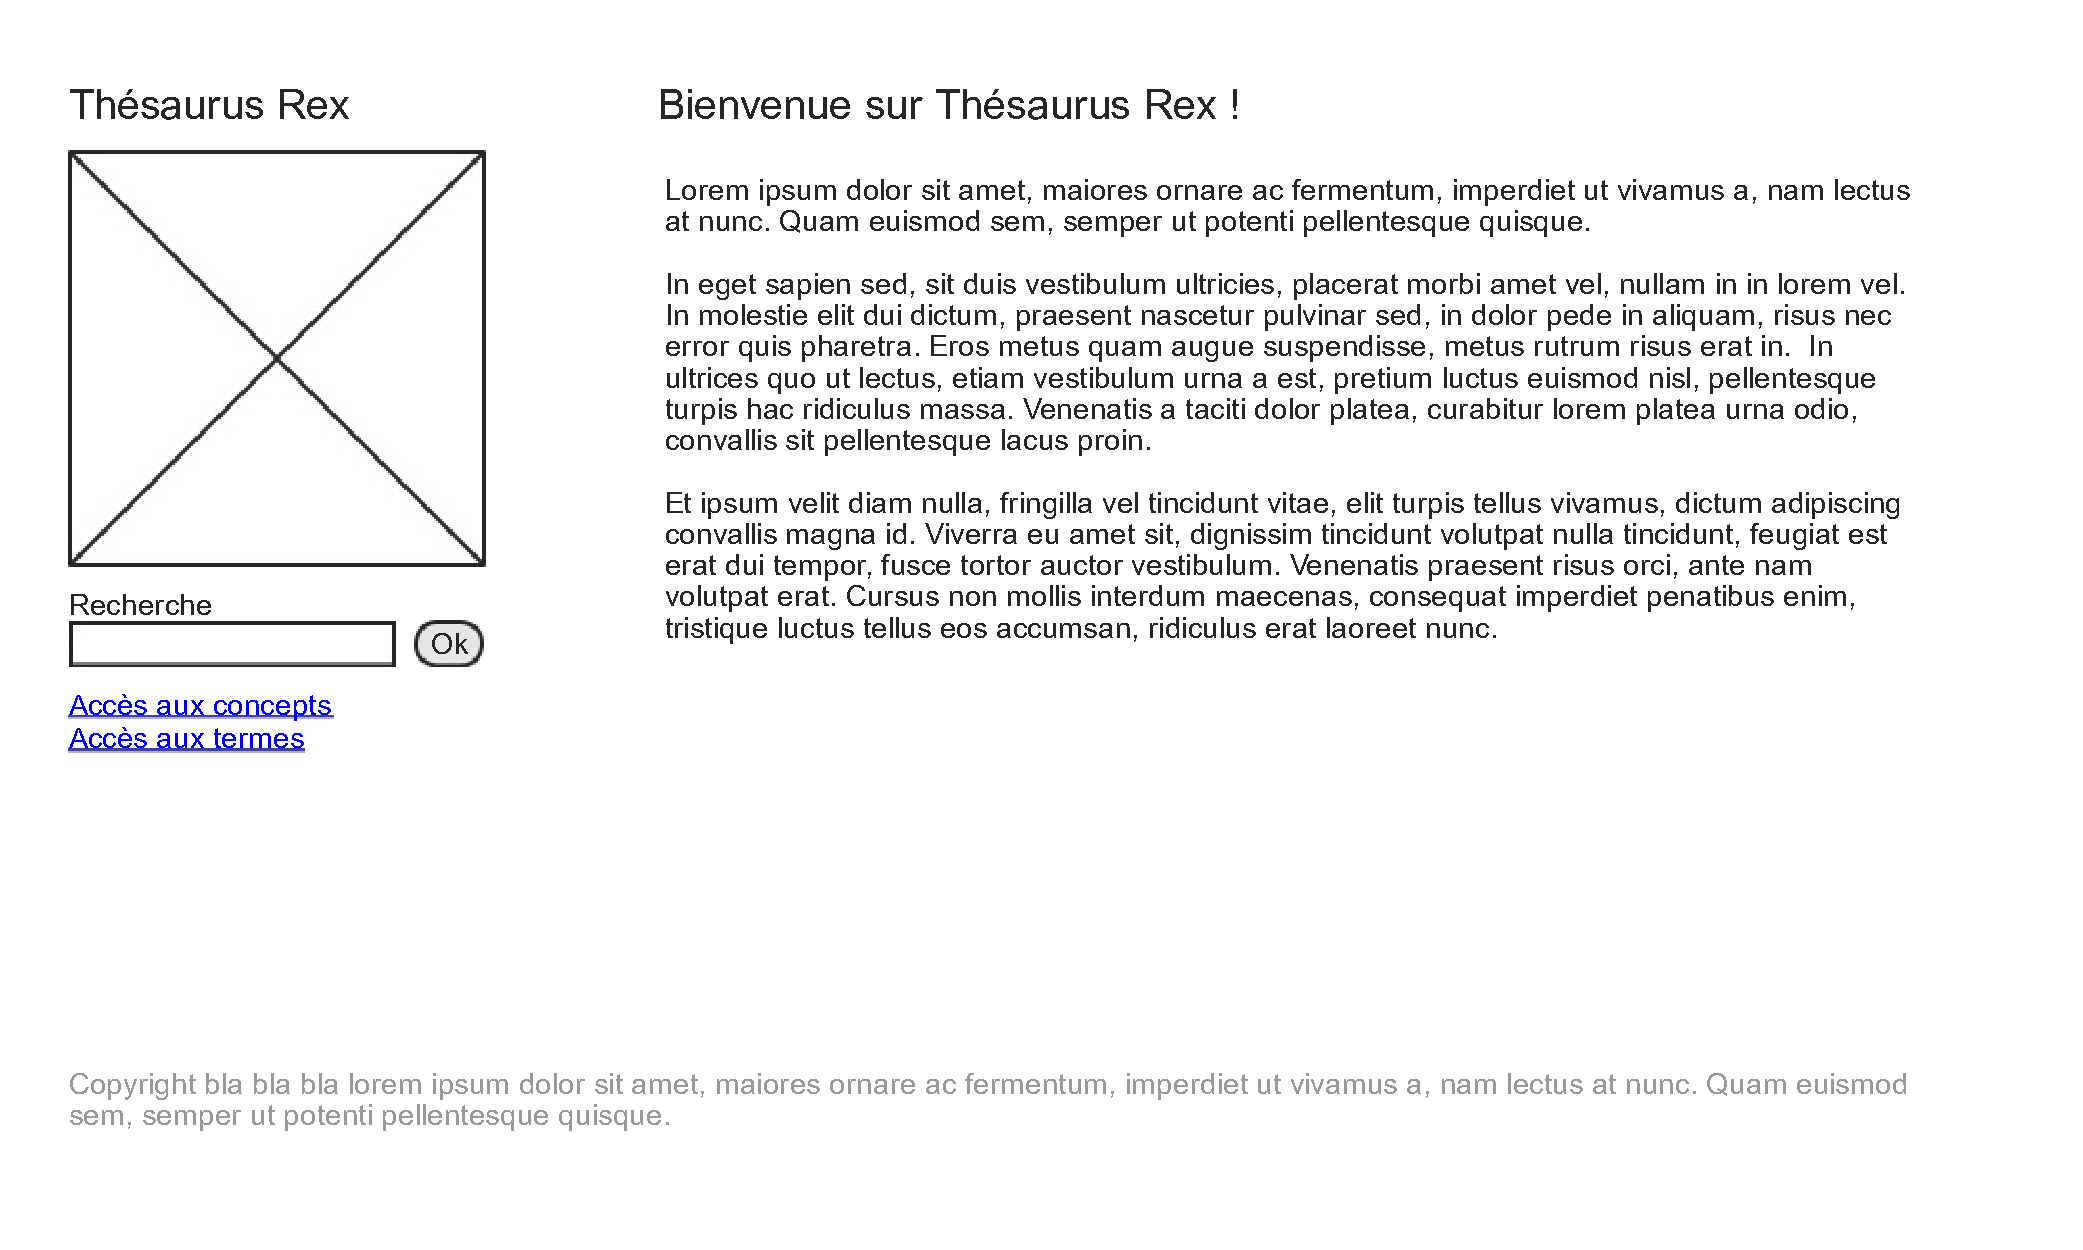
\includegraphics[width=\textwidth]{files/template_accueil}
\end{center}
\caption{Template de la page d'accueil de Thésaurus Rex.}
\end{figure}

\subsubsection{Vue hiérarchique des concepts}
\begin{figure}[H]
\begin{center}
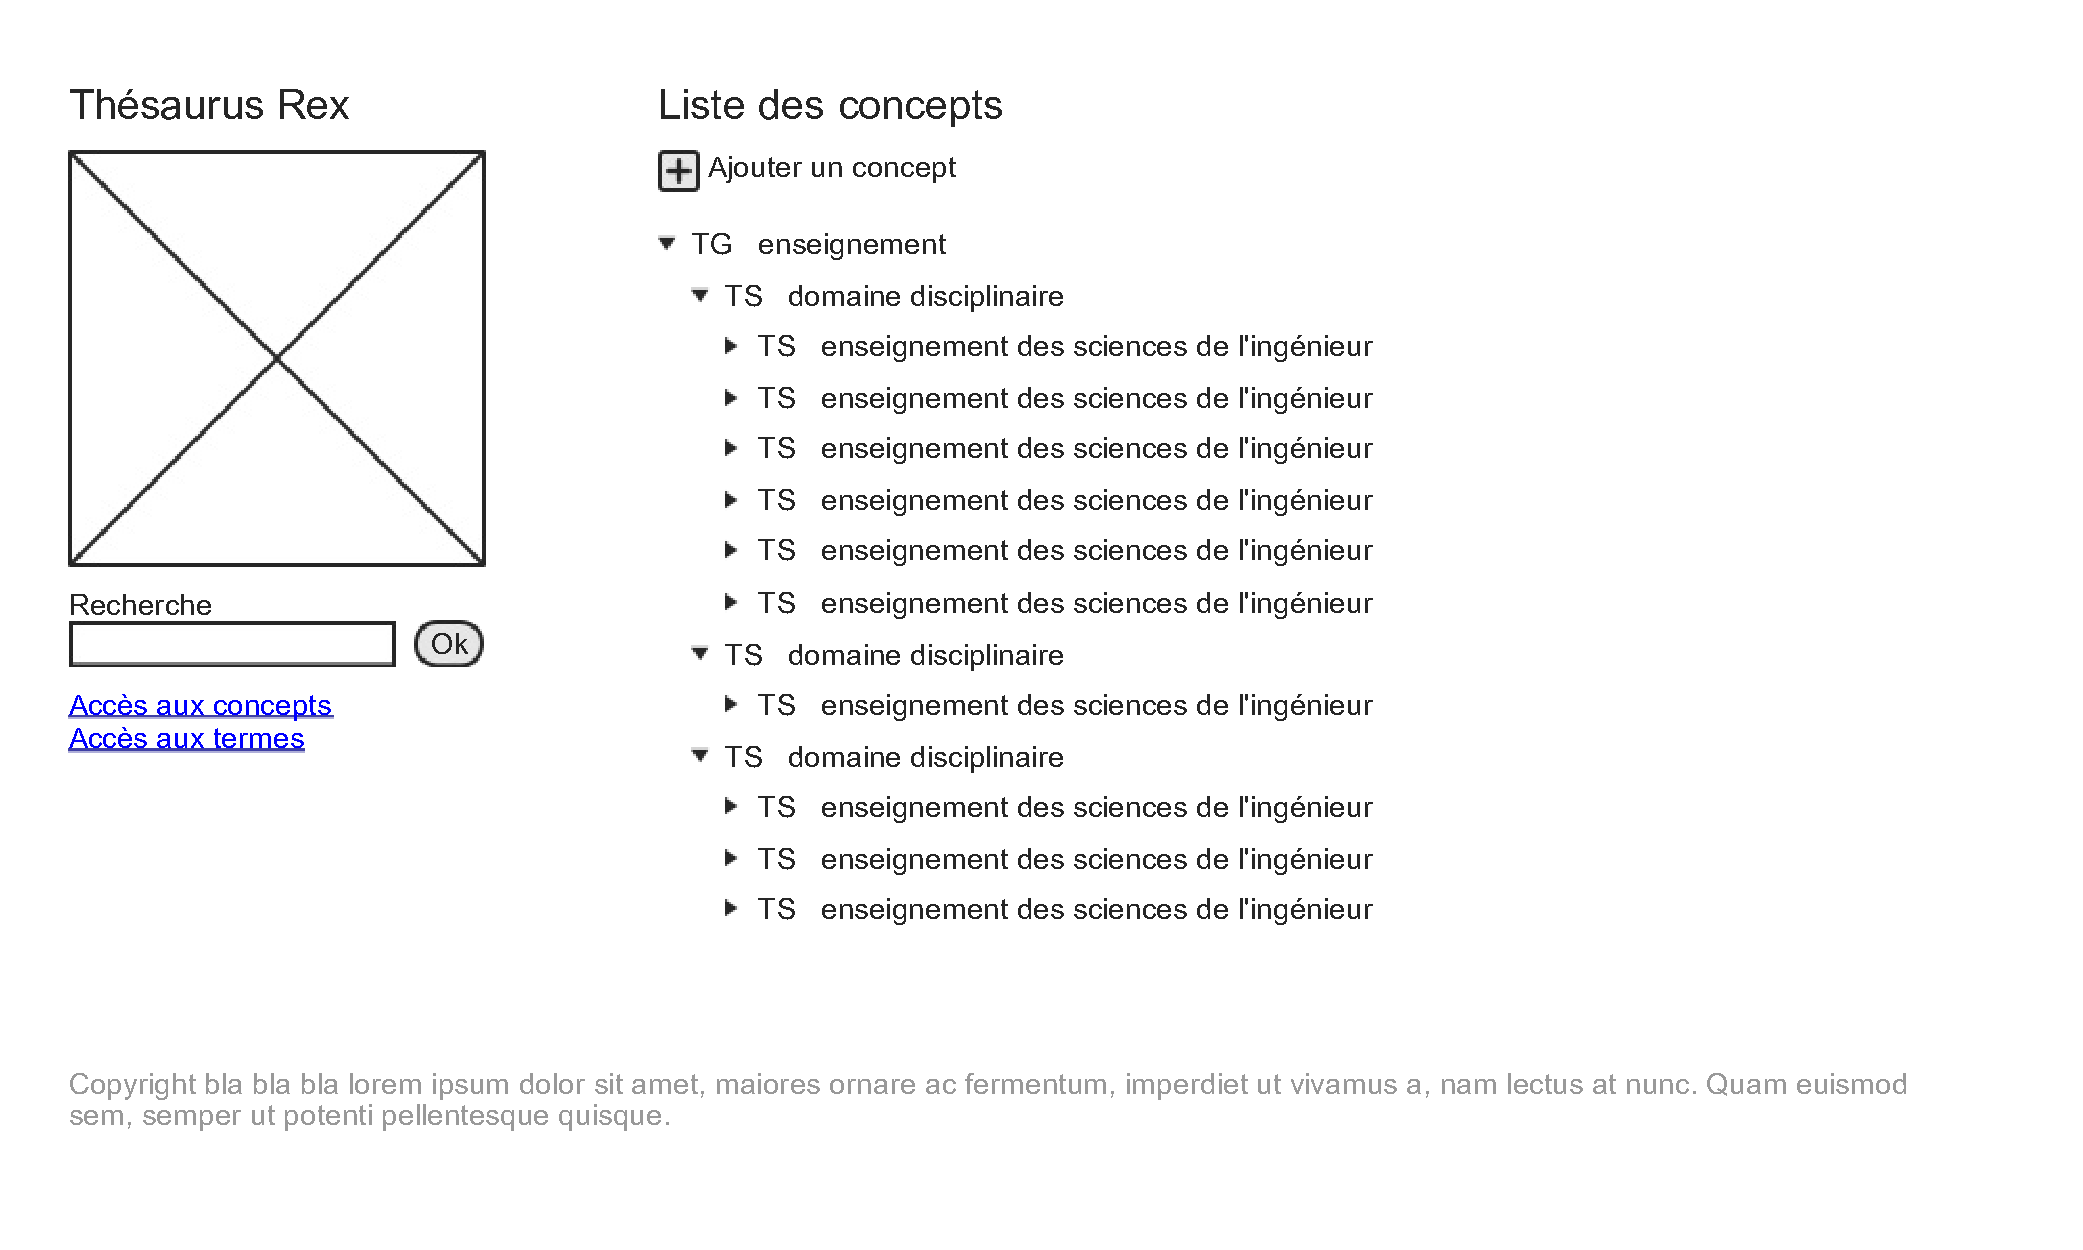
\includegraphics[width=\textwidth]{files/template_concepts}
\end{center}
\caption{Template de la vue hiérarchique des concepts.}
\end{figure}

\subsubsection{Visualisation d'un concept}
\begin{figure}[H]
\begin{center}
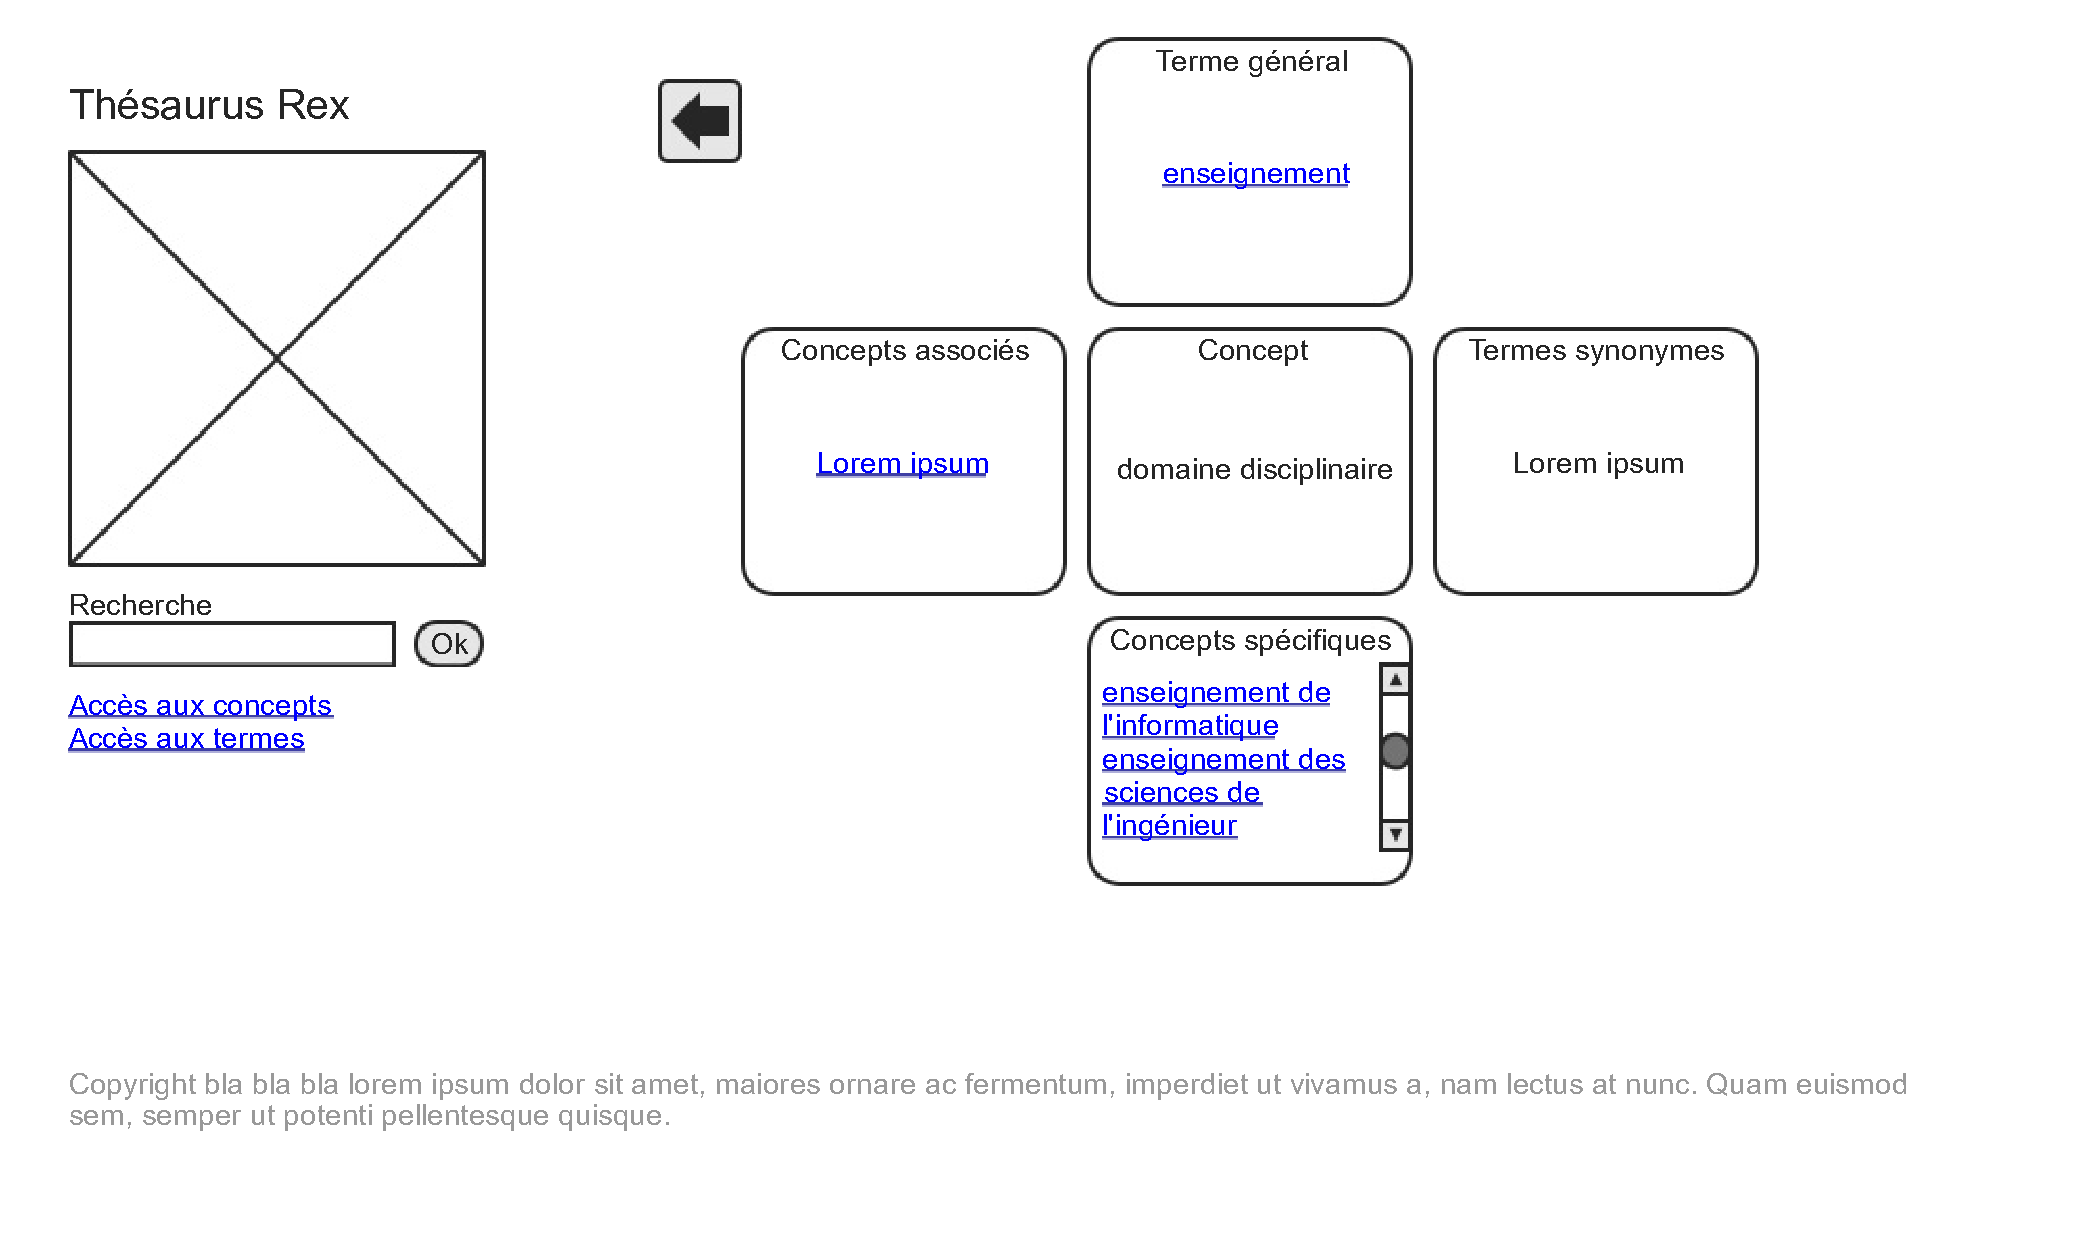
\includegraphics[width=\textwidth]{files/template_concept}
\end{center}
\caption{Template d'affichage d'un concept.}
\end{figure}

\subsubsection{Ajout / Édition d'un concept}
\begin{figure}[H]
\begin{center}
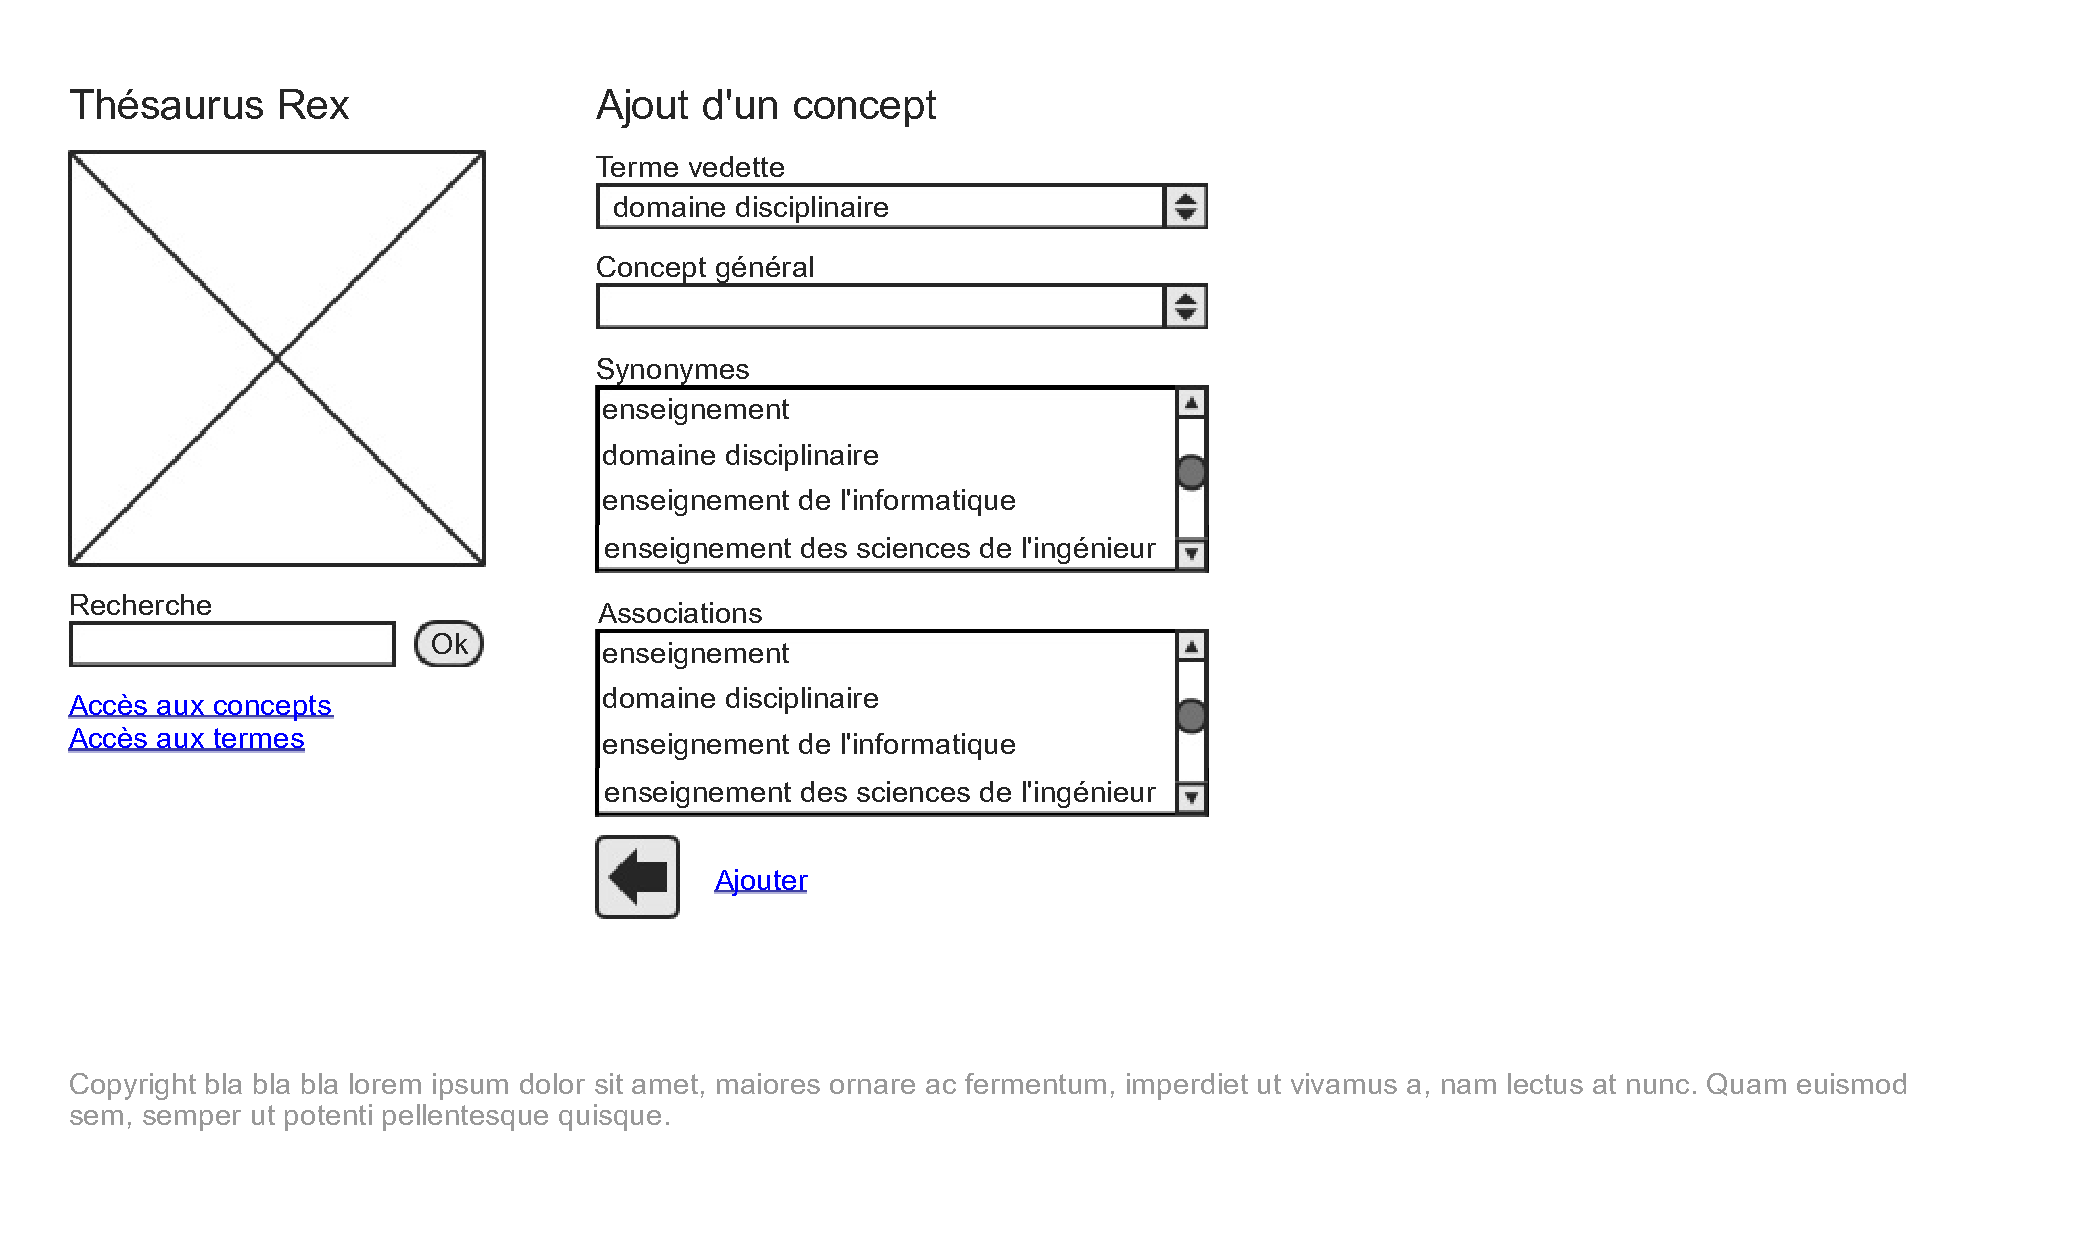
\includegraphics[width=\textwidth]{files/template_concept_add}
\end{center}
\caption{Template du formulaire d'ajout d'un concept.}
\end{figure}
\begin{figure}[H]
\begin{center}
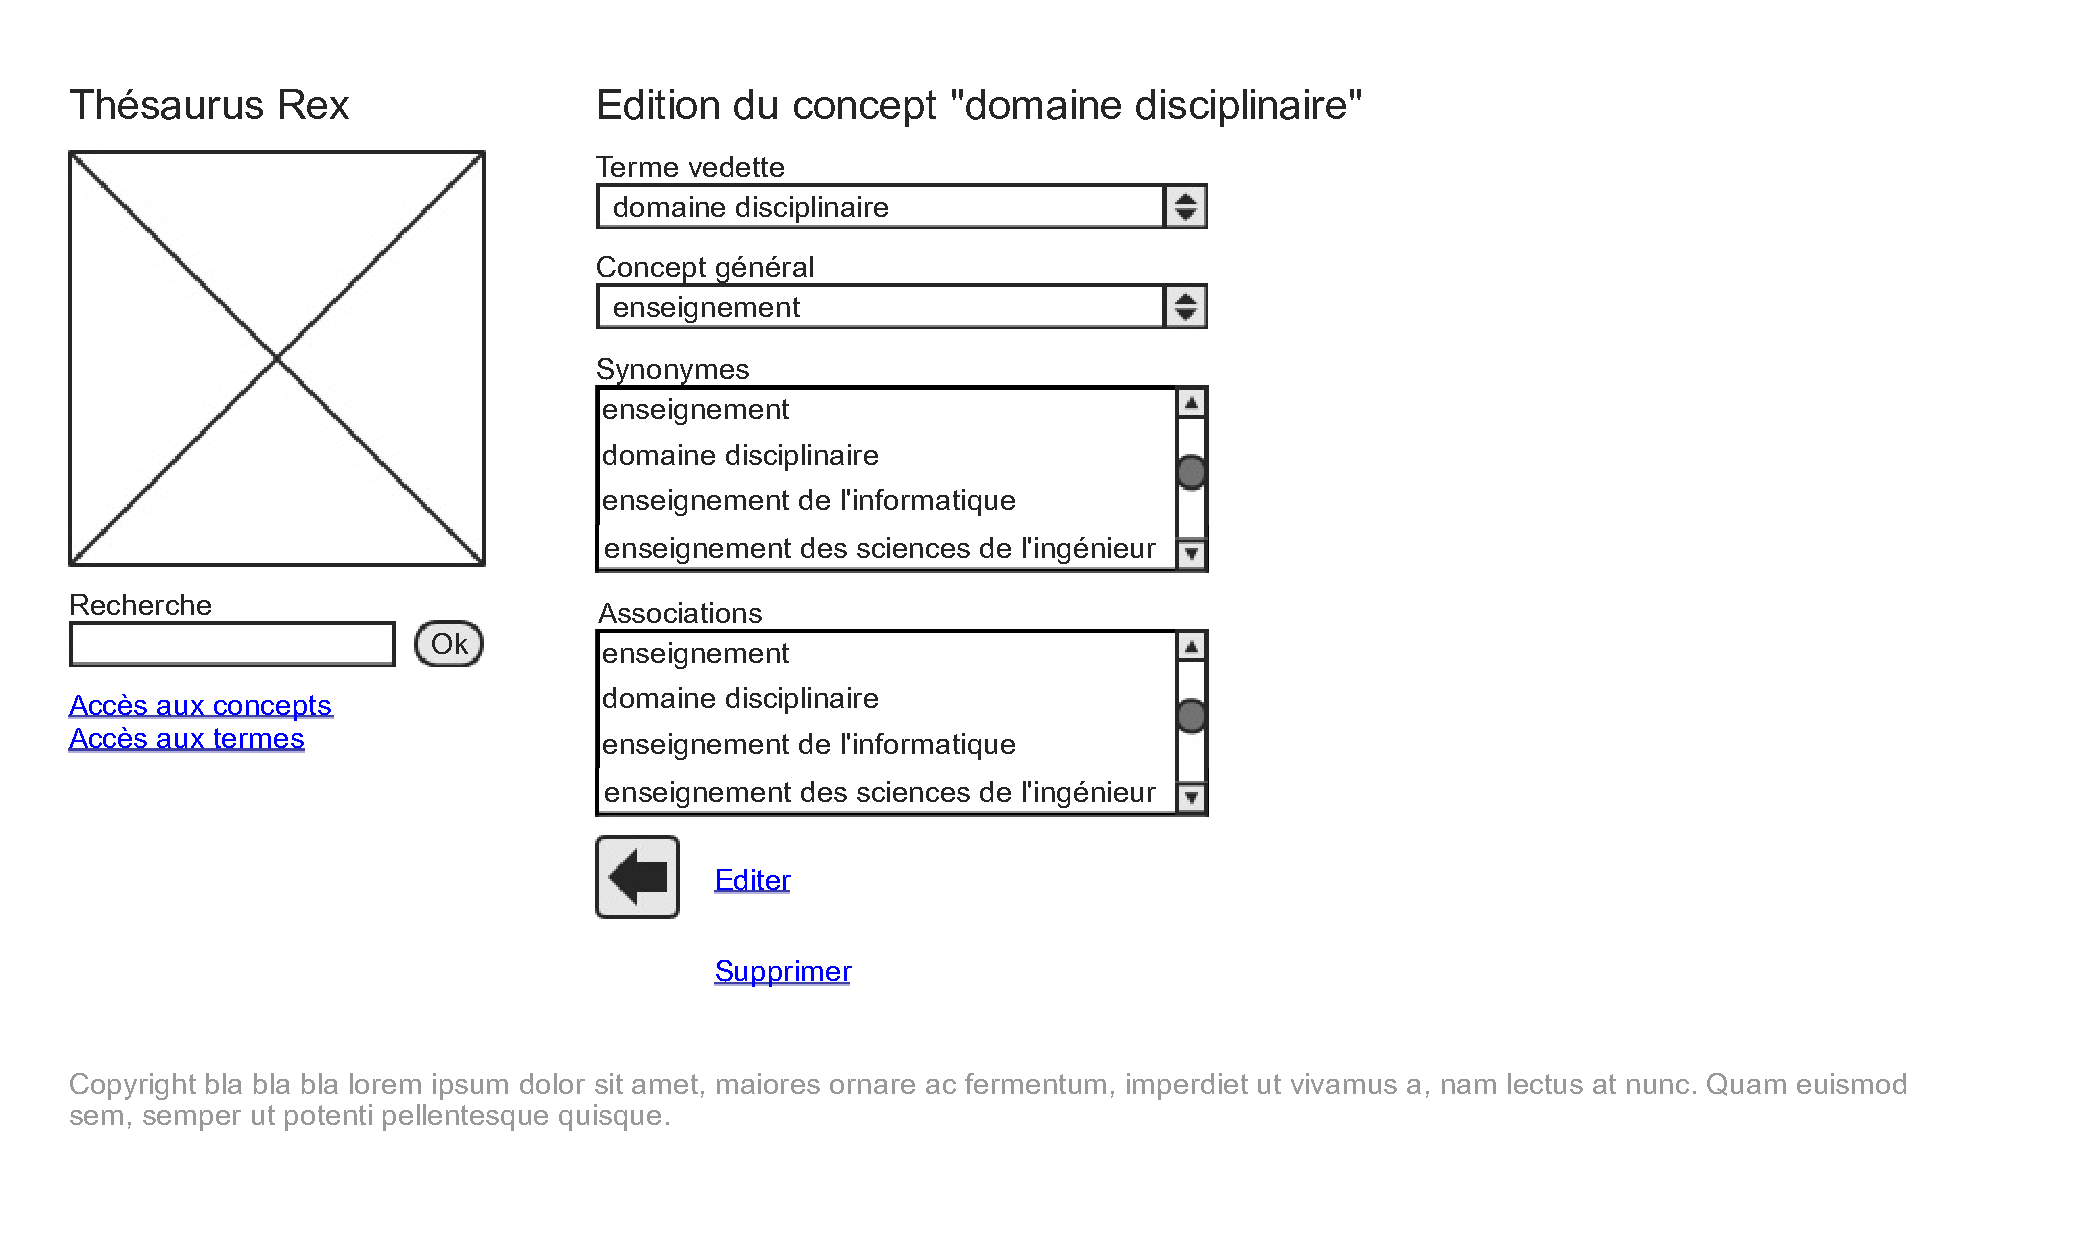
\includegraphics[width=\textwidth]{files/template_concept_edit}
\end{center}
\caption{Template du formulaire d’édition d'un concept.}
\end{figure}

\subsubsection{Liste des termes}
\begin{figure}[H]
\begin{center}
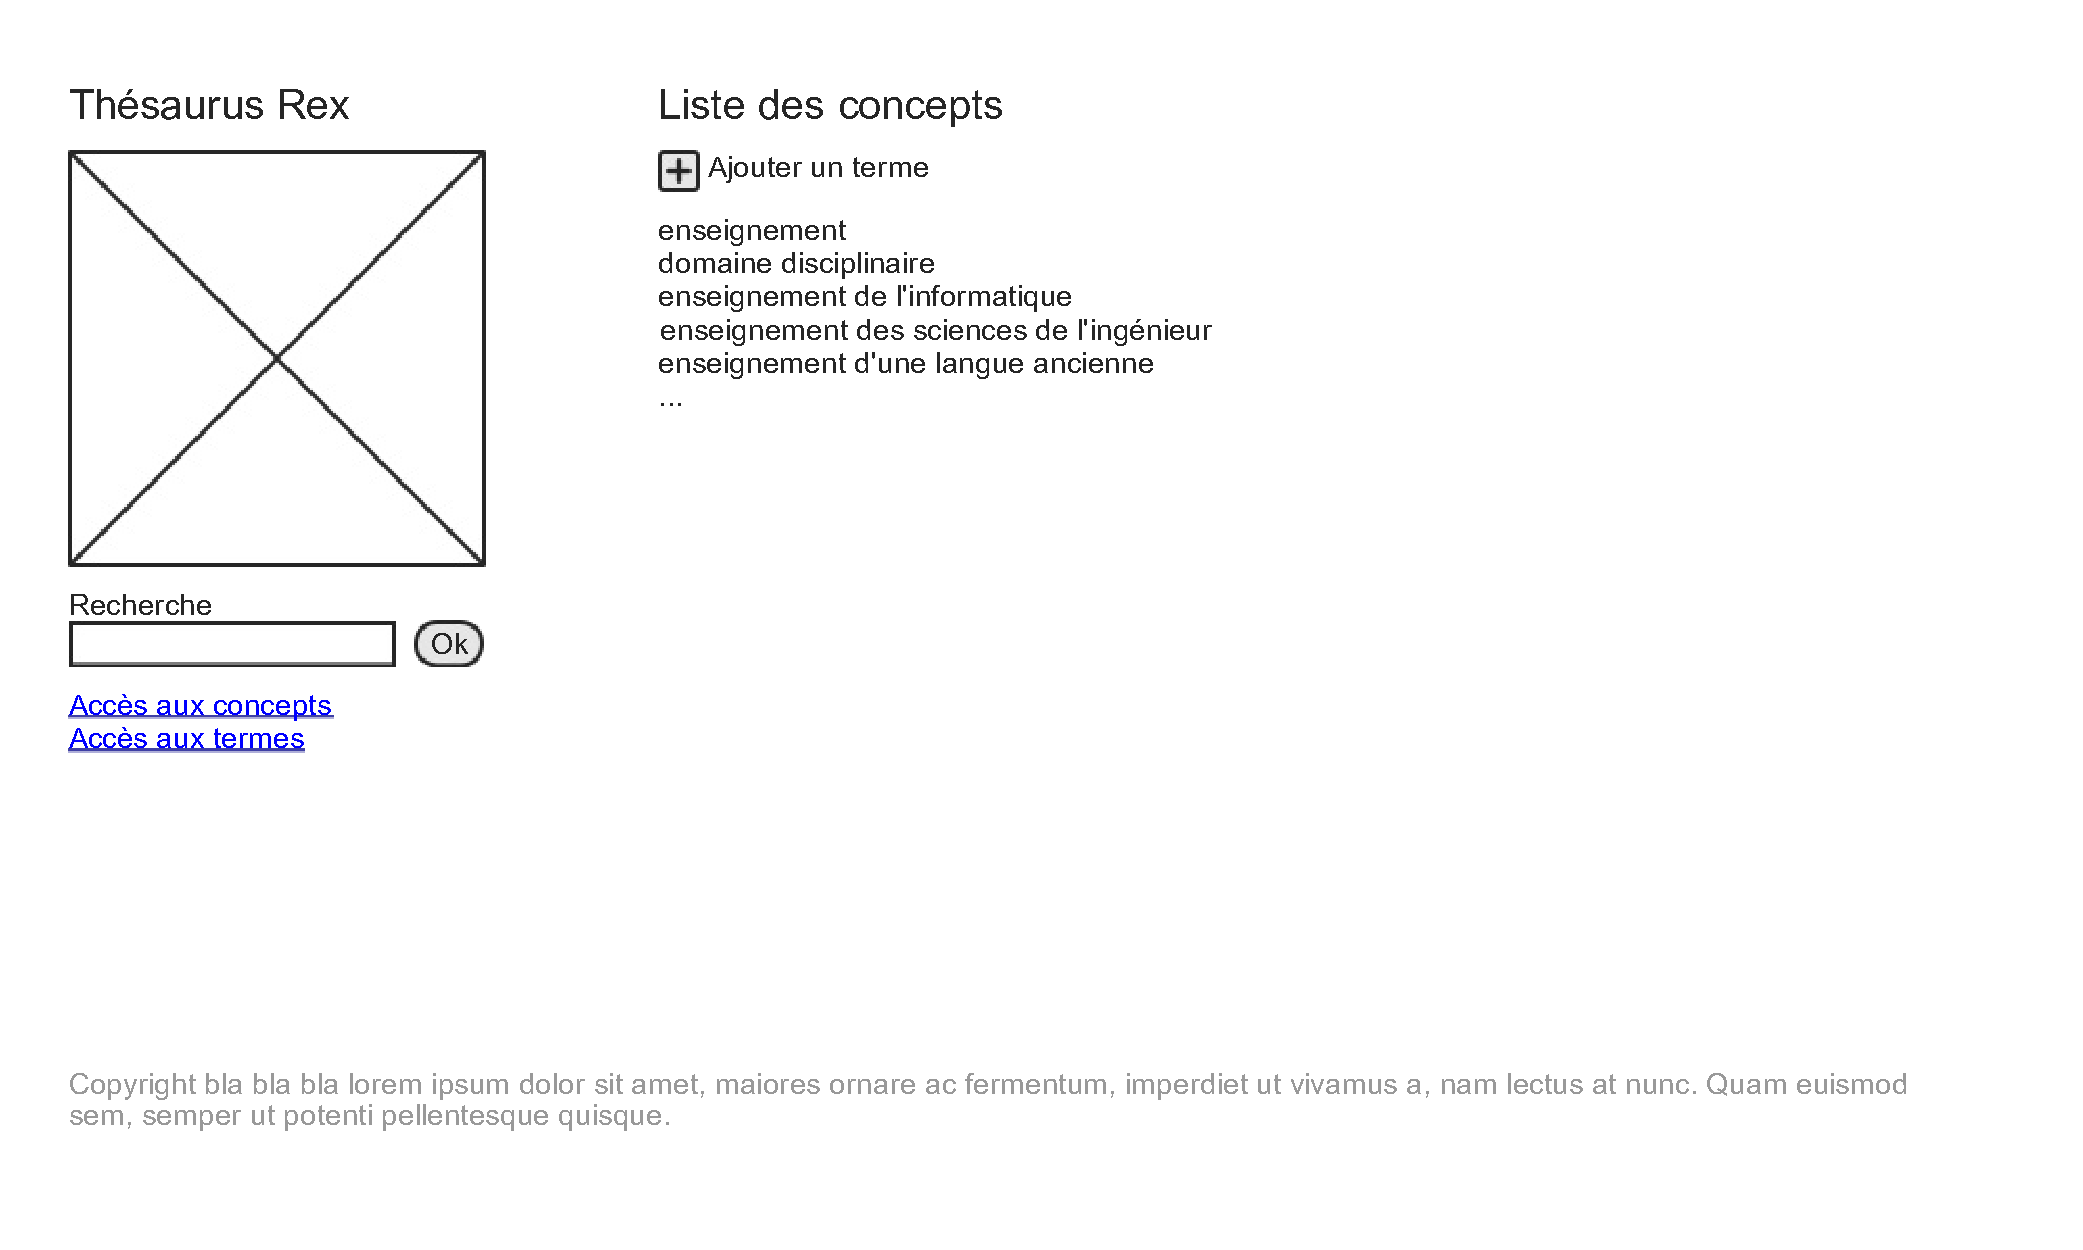
\includegraphics[width=\textwidth]{files/template_termes}
\end{center}
\caption{Template de visualisation des termes.}
\end{figure}

\subsubsection{Édition d'un terme}
\begin{figure}[H]
\begin{center}
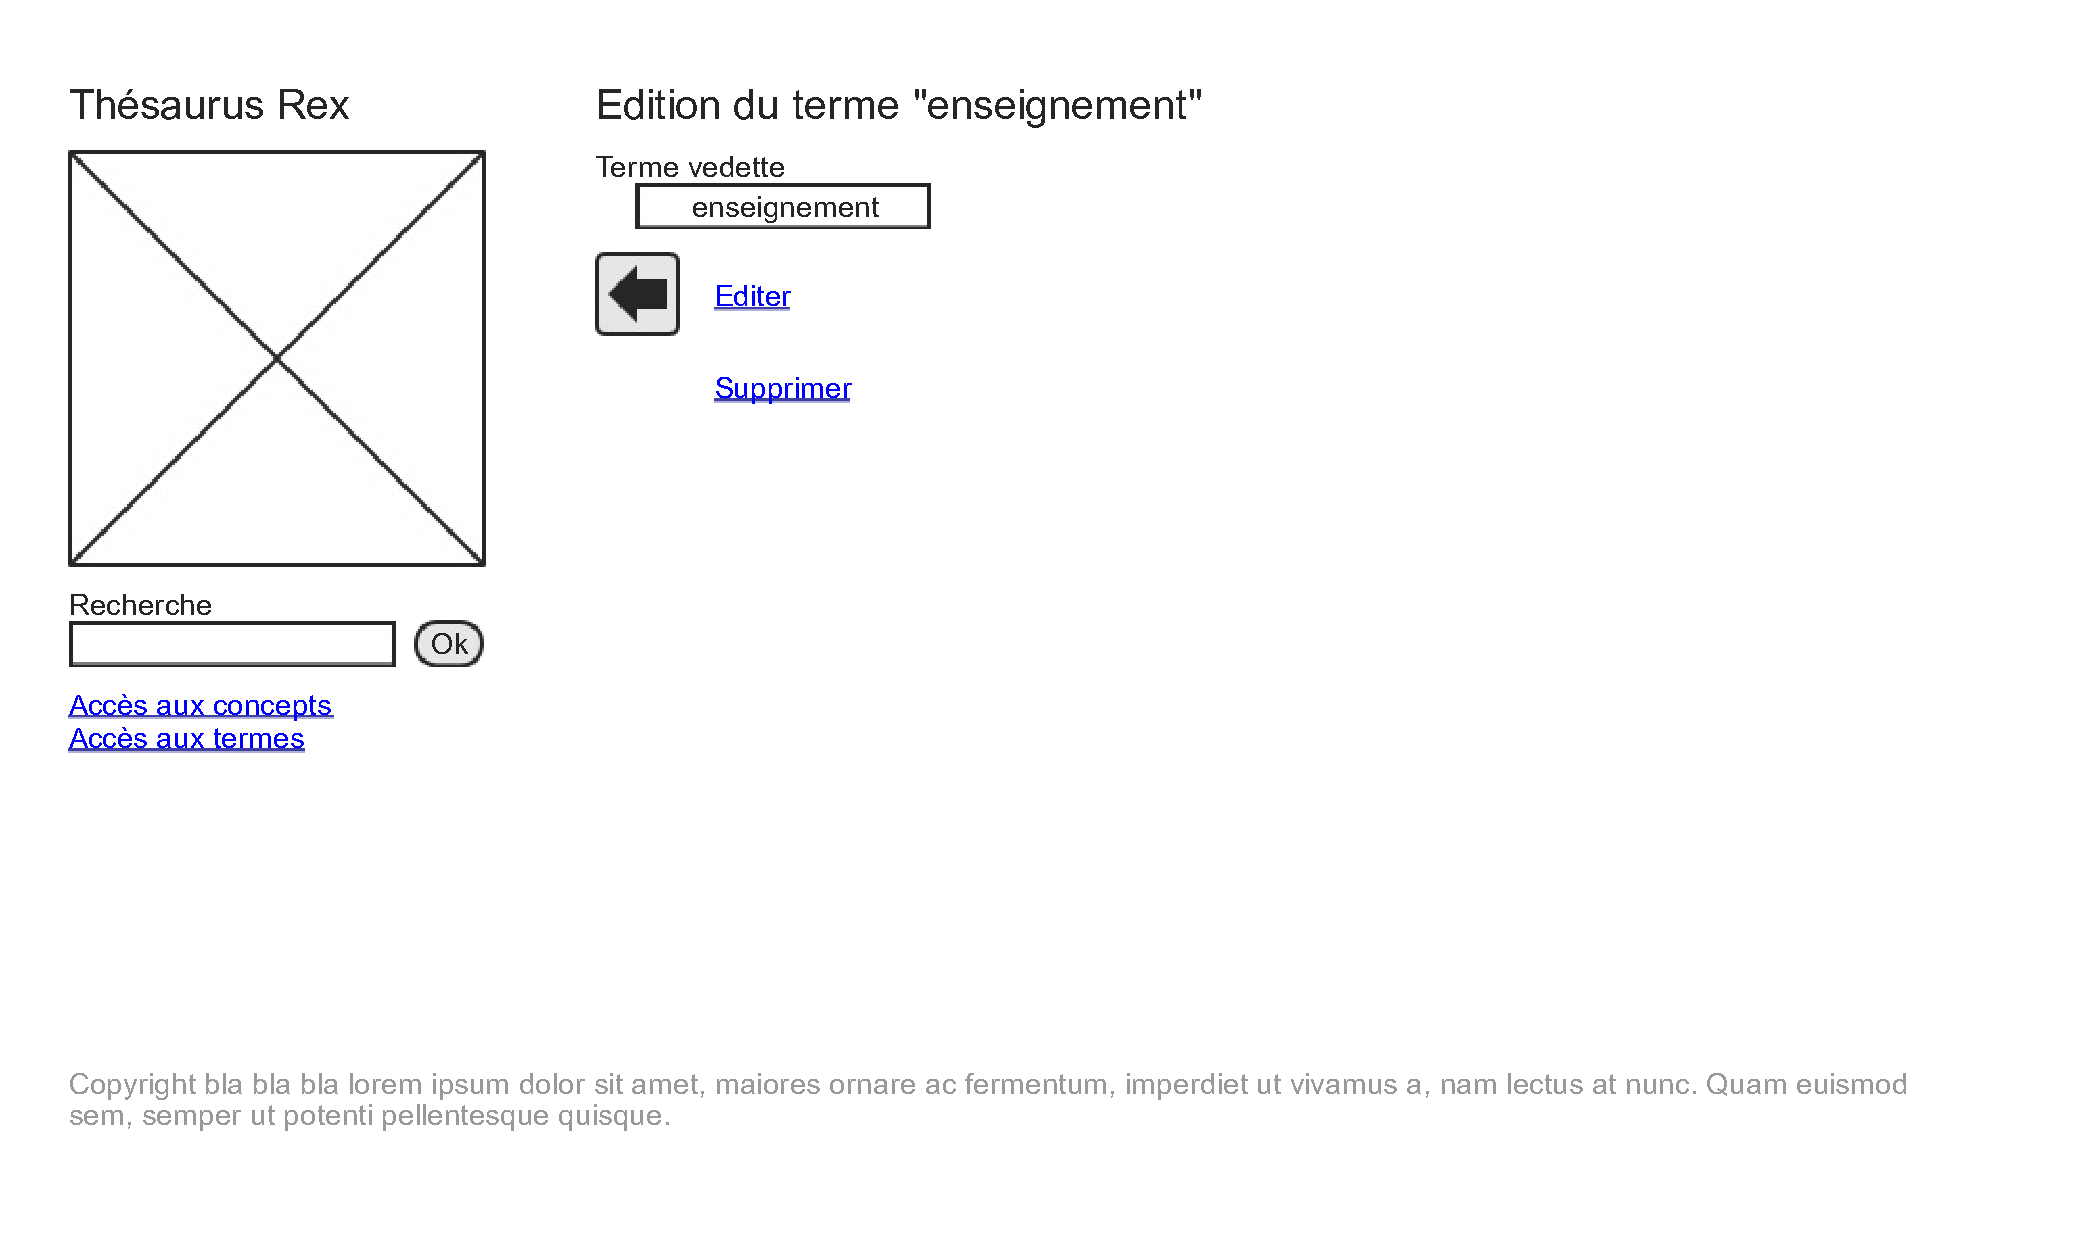
\includegraphics[width=\textwidth]{files/template_terme_edit}
\end{center}
\caption{Template du formulaire d'ajout d'un concept.}
\end{figure}


\subsection{Framework}